% $Header$

\documentclass{beamer}

% This file is a solution template for:

% - Talk at a conference/colloquium.
% - Talk length is about 20min.
% - Style is ornate.



% Copyright 2004 by Till Tantau <tantau@users.sourceforge.net>.
%
% In principle, this file can be redistributed and/or modified under
% the terms of the GNU Public License, version 2.
%
% However, this file is supposed to be a template to be modified
% for your own needs. For this reason, if you use this file as a
% template and not specifically distribute it as part of a another
% package/program, I grant the extra permission to freely copy and
% modify this file as you see fit and even to delete this copyright
% notice. 


\mode<presentation>
{
  \usetheme{Warsaw}
  % or ...

  \setbeamercovered{transparent}
  % or whatever (possibly just delete it)
}


\usepackage[english]{babel}
% or whatever

\usepackage[utf8]{inputenc}
% or whatever

\usepackage{tikz}
\usetikzlibrary{arrows, shapes}

\usepackage{times}
\usepackage[T1]{fontenc}
% Or whatever. Note that the encoding and the font should match. If T1
% does not look nice, try deleting the line with the fontenc.

%\newtheorem{definition}{Definition}

\title% (optional, use only with long paper titles)
{Consensus and replication}

\subtitle
{From impossibility to production}

\author[Alexander Kharitonov]{Alexander Kharitonov \\ \texttt{a@cmpxchg.me}}
\date{Yandex science seminar, 22 Mar 2012}

%\author[Author, Another] % (optional, use only with lots of authors)
%{F.~Author\inst{1} \and S.~Another\inst{2}}
% - Give the names in the same order as the appear in the paper.
% - Use the \inst{?} command only if the authors have different
%   affiliation.
%\institute[Yandex]
%{
%    Yandex LLC
%}

%\institute[Universities of Somewhere and Elsewhere] % (optional, but mostly needed)
%{
%  \inst{1}%
%  Department of Computer Science\\
%  University of Somewhere
%  \and
%  \inst{2}%
%  Department of Theoretical Philosophy\\
%  University of Elsewhere}
% - Use the \inst command only if there are several affiliations.
% - Keep it simple, no one is interested in your street address.

%\date[CFP 2003] % (optional, should be abbreviation of conference name)
%{Conference on Fabulous Presentations, 2003}
% - Either use conference name or its abbreviation.
% - Not really informative to the audience, more for people (including
%   yourself) who are reading the slides online

\subject{Distributed systems}
% This is only inserted into the PDF information catalog. Can be left
% out. 



% If you have a file called "university-logo-filename.xxx", where xxx
% is a graphic format that can be processed by latex or pdflatex,
% resp., then you can add a logo as follows:

% \pgfdeclareimage[height=0.5cm]{university-logo}{university-logo-filename}
% \logo{\pgfuseimage{university-logo}}



% Delete this, if you do not want the table of contents to pop up at
% the beginning of each subsection:
\AtBeginSubsection[]
{
  \begin{frame}<beamer>{Outline}
    \tableofcontents[currentsection,currentsubsection]
  \end{frame}
}


% If you wish to uncover everything in a step-wise fashion, uncomment
% the following command: 

%\beamerdefaultoverlayspecification{<+->}


\begin{document}

\begin{frame}
  \titlepage
\end{frame}

\begin{frame}{Outline}
  \tableofcontents
  % You might wish to add the option [pausesections]
\end{frame}


% Structuring a talk is a difficult task and the following structure
% may not be suitable. Here are some rules that apply for this
% solution: 

% - Exactly two or three sections (other than the summary).
% - At *most* three subsections per section.
% - Talk about 30s to 2min per frame. So there should be between about
%   15 and 30 frames, all told.

% - A conference audience is likely to know very little of what you
%   are going to talk about. So *simplify*!
% - In a 20min talk, getting the main ideas across is hard
%   enough. Leave out details, even if it means being less precise than
%   you think necessary.
% - If you omit details that are vital to the proof/implementation,
%   just say so once. Everybody will be happy with that.

\section{Motivation}
\subsection{High availability and state machine replication}

\begin{frame}{Introduction}
  \begin{itemize}
  \item We want to build systems that work despite some number of failing components.
  \item Particularly want no single points of failure.
  \item Hence such systems are necessarily distributed.
  \item Unfortunately, distributed systems are very hard to reason about.
  \item Separate the resilience and application logic: treat the system as a state machine.
  \end{itemize}
\end{frame}

\begin{frame}{State machine}
  \begin{definition}
    A state machine is a tuple $S = (Q, \varphi, I, O)$, where $Q$ is the set of states, $\varphi\colon Q \times I \to Q \times O$ is the state transition function, $I$ is the input command set and $O$ is the output set.
  \end{definition}
  Some (trivial) notes:
  \begin{itemize}
  \item $Q$ is not necessarily finite, so e.g. a Turing machine is a valid state machine by our definition.
  \item $\varphi$ is deterministic.
  \end{itemize}
\end{frame}

\begin{frame}{State machine example: a read-write register}
  \begin{definition}
    A read-write register is essentially a memory cell that can hold a single natural number (or be empty).
    \begin{itemize}
      \item $Q = \mathbb{N} \cup \{ \bot \}$
      \item $I = \textsc{read} \cup \{ \textsc{write}(i) \mid i \in \mathbb{N} \}$
      \item $O = \textsc{ok} \cup Q$
      \item $\varphi(q, \textsc{read}) = (q, q)$
      \item $\varphi(q, \textsc{write}(i)) = (i, \textsc{ok})$
    \end{itemize}
  \end{definition}
\end{frame}

%\begin{frame}{Sequential specifications and linearizability}
%  \begin{itemize}
%    \item A state machine is a complete sequential specification of the system that it models.

\begin{frame}{State machine replication}
  \begin{itemize}
    \item In real life computers crash, power goes out etc. Systems fail.
    \item To remain available despite faults the system must be replicated.
  \end{itemize}
\end{frame}

\begin{frame}{State machine replication: the setting}
  \begin{itemize}
    \item There is a set of clients $C$ and a set of replicas $R$ which communicate over the network.
    \item Some protocol provides the clients with an abstraction of a single state machine they all interact with (backed by $R$).
    \item Can have various consistency guarantees depending on the system model and on kinds of tolerated failures, e.g. linearizability, single-client FIFO, eventual consistency etc.
    \item Tolerates some kinds of replica failures (again, depends on the system model and synchrony assumptions).
  \end{itemize}
\end{frame}

\subsection{Replication, atomic broadcast and consensus}

\begin{frame}{On failure model and synchrony assumptions}
  We will assume the following:
  \begin{itemize}
    \item Failures are crash-stop: no crashed replica ever recovers. This is for simplicity, practically everything can be adapted to the crash-recovery setting.
    \item The system is initially asynchronous. That means no bounds on message losses and delays, no bounds on the relative speed of the processes, no shared clocks whatsoever.
    \item There is an (unknown to the processes) Global Stabilization Time, after which no processes crash and message delays and clock drift become bounded (but bounds remain unknown).
  \end{itemize}
\end{frame}

\begin{frame}{On failure model and synchrony assumptions (cont'd)}
  \begin{itemize}
    \item Actually, things need not to remain stable forever after GST. The only requirement for liveness is for the stability period to be long enough for a step of replication to complete.
    \item Under these assumptions we will construct systems that tolerate up to $\lfloor\frac{n-1}{2}\rfloor$ failures in a system of $n$ processes.
  \end{itemize}
  \begin{definition}
    With respect to some execution of some distributed algorithm, a \alert{correct} process is a process that did not crash in that execution.
  \end{definition}
\end{frame}

\begin{frame}{Atomic broadcast}
  \begin{definition}
    Atomic broadcast is a group communication primitive providing two operations:
    \begin{itemize}
      \item $\textsc{broadcast}(m)$ -- send a message $m$ to everyone in the group
      \item $\textsc{deliver}(m)$ -- deliver a message.
    \end{itemize}
    with the following guarantees:
  \end{definition}
\end{frame}

\begin{frame}{Atomic broadcast guarantees}
  \begin{enumerate}
    \item If a process \textsc{deliver}s $m$, then all \alert{correct} processes eventually (after GST) deliver $m$.
    \item A process can only \textsc{deliver} a message that has been \textsc{broadcast} by some process.
    \item No two processes \textsc{deliver} any two messages in different orders.
    \item If a correct process \textsc{broadcast}s $m$, then all \alert{correct} processes eventually \textsc{deliver} $m$.
  \end{enumerate}
  Guarantees $2$ and $3$ are \alert{uniform safety} properties that hold for \alert{all} processes, including the faulty ones.
\end{frame}

\begin{frame}{State machine replication via atomic broadcast}
  \begin{itemize}
    \item With atomic broadcast state machine replication becomes easy, as it delivers a uniform sequence of message to all replicas.
    \item A na\"ive but working approach to SMR would be for each client to maintain a copy of the state machine, \textsc{broadcast} its commands and apply commands in the order they are \textsc{deliver}ed.
  \end{itemize}
\end{frame}

\begin{frame}{Consensus}
  \begin{definition}
    Consensus is a distributed agreement primitive defined by two operations
    \begin{itemize}
      \item $\textsc{propose(v)}$ -- propose a value $v$
      \item $\textsc{decide(v)}$ -- decide that $v$ has been chosen
    \end{itemize}
    satisfying:
    \begin{enumerate}
      \item If a process \textsc{decide}s $v$ then some process \textsc{propose}d $v$
      \item \textsc{decide} \alert{never} decides two different values (in a single consensus execution, there are no two \textsc{decide} calls returning different values).
      \item If any correct process \textsc{propose}s a value then eventually all correct processes \textsc{decide} some value.
    \end{enumerate}
  \end{definition}
\end{frame}

\begin{frame}{Consensus is equivalent to atomic broadcast}{Consensus via atomic broadcast}
  \begin{enumerate}
    \item To \textsc{propose} a value $v$, \textsc{broadcast}($v$).
    \item \textsc{decide} on a first value \textsc{deliver}ed.
  \end{enumerate}
\end{frame}

\begin{frame}{Consensus is equivalent to atomic broadcast}{Atomic broadcast via consensus}
  \begin{itemize}
    \item Run a series of consensus instances indexed by $\mathbb{N}$.
    \item Intuitively, consensus in instance $i$ on a value $m$ means that $m$ is the $i$th value in the broadcast sequence.
    \item To \textsc{broadcast} a value $v$, pick the lowest instance on which consensus is unknown and \textsc{propose} $v$. Repeat until success.
    \item \textsc{deliver} values in the order of their instance numbers.
  \end{itemize}
\end{frame}

\section{FLP impossibility}
\subsection{The result}
\begin{frame}{FLP impossibility theorem}
  \begin{theorem}[Fischer, Lynch, Patersson 1985]
    Consensus is impossible to achieve in a sufficiently asynchronous system with even one crashed process.
  \end{theorem}

  \begin{itemize}
    \item The actual result is stronger. It asserts the impossibility of the weakest form of consensus possible, namely when there \emph{exists} a process that \textsc{decide}s.
    \item To prove it, we need to specify the computation model more precisely...
  \end{itemize}
\end{frame}

\subsection{The model}
\begin{frame}{The message system}
  Let $\mathbb{P}$ denote the set of processes in our asynchronous system. The processes communicate by sending messages to one another from some fixed universe $\mathbb{M}$ via the \emph{message system}.
\end{frame}

\begin{frame}{The message system}
  \begin{definition}
    The message system is a multiset of sent but not yet delivered messages, called the \emph{message buffer}, with the following two operations:
    \begin{itemize}
      \item $\textsc{send}(p, m)$ -- places $(p,m)$ in the message buffer.
      \item $\textsc{receive}(p)$ -- non-deterministically deletes some message $(p, m)$ from the buffer and returns $m$, or returns $\varnothing$ leaving the buffer unchanged.
    \end{itemize}
  The only constraint on the non-determinism of \textsc{receive} is that if there is some $(p, m)$ in the message buffer then there can be no infinite sequence of $\textsc{receive}(p)$ operations all returning $\varnothing$. The message system is thus an abstraction of lossless communication links with arbitrary delays and reordering.
  \end{definition}
\end{frame}

\begin{frame}{The processes}
  \begin{itemize}
    \item A process is a state machine with $I = \mathbb{M} \cup \{ \varnothing \}$ and $O = (\mathbb{P} \times \mathbb{M})^*$.
    \item Each process $p$ has a one-bit read-only \alert{input register} $x_p$ and an \alert{output register} $y_p$ with values in $\{ \bot, 0, 1\}$. Each state $q \in Q$ includes the states of these two registers and is otherwise arbitrary.
    \item The states in which $y_p \ne \bot$ are \alert{decision states}.
    \item $y_p$ is \alert{write-once}: $y_p$ cannot be changed once the process is in a decision state.
    \item In an \alert{initial state}, $y_p = \bot$.
  \end{itemize}
\end{frame}

\begin{frame}{System configuration}
  \begin{itemize}
    \item A configuration $C$ of the system is the set $\{ q_p \mid p \in \mathbb{P} \}$ of current process states together with the contents of the message buffer.
    \item An \alert{initial configuration} is that in which each process is in some initial state and the message buffer is empty.
  \end{itemize}
\end{frame}

\begin{frame}{System step}
  A step takes the system from one configuration to another. It consists of a following sequence of actions performed atomically by some process $p$.
  \begin{itemize}
    \item $m := \textsc{receive}(p)$
    \item $(q_p, o) := \varphi_p(q_p, m)$
    \item $\textsc{send}(p', m')$ for every $(p', m')$ in $o$.
  \end{itemize}
  The entire step is determined by the pair $e = (p, m)$ that gets \textsc{receive}d. We will henceforth call $e$ an \alert{event} and denote the configuration that results from applying $e$ to $C$ by $e(C)$.
\end{frame}

\begin{frame}{System evolution}
  \begin{itemize}
    \item A \alert{schedule} from $C$ is a sequence $\sigma$ of events that can be applied, in turn, starting from $C$.
    \item A \alert{run} from $C$ is a sequence of steps corresponding to a schedule from $C$.
    \item If $\sigma$ is finite, then let $\sigma(C)$ denote the configuration resulting from applying $\sigma$ to $C$. We say that $\sigma(C)$ is \alert{reachable} from $C$.
    \item A configuration reachable from some initial configuration is said to be \alert{accessible}. We will only consider accessible configurations hereafter.
  \end{itemize}
\end{frame}

\subsection{The proof}
\begin{frame}{Disjoint schedule commutativity}
  \begin{lemma}
    Consider two schedules $\sigma_1, \sigma_2$ from some configuration $C$. If the sets of processes taking steps in $\sigma_1$ and $\sigma_2$ are disjoint, then $\sigma_1(\sigma_2(C)) = \sigma_2(\sigma_1(C)) = C'$.
  \end{lemma}
  \begin{proof}
    Obvious.
  \end{proof}
\end{frame}

\begin{frame}{Disjoint schedule commutativity}
  \begin{figure}[!h]
  \centering
  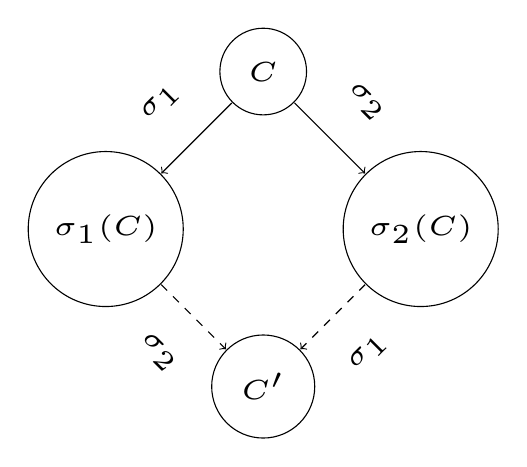
\begin{tikzpicture}[transform shape, scale=2]
    \tikzstyle{every node} = [shape=circle]
    \node (a) [draw] at (1, 2) {\tiny $C$};
    \node (b) [draw] at (0, 1) {\tiny $\sigma_1(C)$};
    \node (c) [draw] at (2, 1) {\tiny $\sigma_2(C)$};
    \node (d) [draw] at (1, 0) {\tiny $C'$};
      \draw [->] (a) -- (b) node[pos=.5,sloped,above] {\tiny $\sigma_1$};
      \draw [->] (a) -- (c) node[pos=.5,sloped,above] {\tiny $\sigma_2$};
      \draw [dashed, ->] (b) -- (d) node[pos=.5,sloped,below] {\tiny $\sigma_2$};
      \draw [dashed, ->] (c) -- (d) node[pos=.5,sloped,below] {\tiny $\sigma_1$};
  \end{tikzpicture}
  \end{figure}
\end{frame}

\begin{frame}{Correctness of a consensus protocol}
  \begin{definition}
    A configuration $C$ has decision value $v \in \{ 0, 1 \}$ if some $p \in \mathbb{P}$ is in a decision state with $y_p = v$.
  \end{definition}
  \begin{definition}
    A consensus protocol is \alert{partially correct} if:
    \begin{itemize}
      \item No accessible configuration has more than one decision value.
      \item $\forall\, v \in \{0, 1\}\,\exists$ accessible configuration with decision value $v$.
    \end{itemize}
  \end{definition}
\end{frame}

\begin{frame}{Correctness of a consensus protocol}
  \begin{itemize}
    \item A process is \alert{nonfaulty} in a run iff it takes infinitely many steps and \alert{faulty} otherwise.
    \item A run is \alert{admissible} iff at most one process is faulty and all messages sent to nonfaulty processes are eventually received.
    \item A run is \alert{deciding} if some process reaches a decision state in it.
    \item A consensus protocol $P$ is \alert{totally correct in spite of one fault} iff it is partially correct and every admissible run is deciding.
  \end{itemize}
\end{frame}

\begin{frame}{Proof outline}
  We want to prove that no partially correct consensus algorithm is totally correct in spite of one fault. We do that in two steps:
  \begin{itemize}
    \item Prove that there exists an initial configuration in which the decision is not predetermined.
    \item Construct an admissible run from that configuration which avoids ever taking a step that would commit it to a decision.
  \end{itemize}
\end{frame}

\begin{frame}{Univalent and bivalent configurations}
  \begin{definition}
    Let $V$ be a set of decision values of configurations reachable from $C$. C is \alert{bivalent} if $|V| = 2$ and \alert{univalent} if $|V| = 1$ ($0$-valent or $1$-valent).
    
    Note that by the total correctness of $P$ $V \ne \varnothing$.
  \end{definition}
  \begin{lemma}
    $P$ has a bivalent initial configuration.
  \end{lemma}
\end{frame}

\begin{frame}{Proof of lemma}
Each initial configuration corresponds to a vector $\{ x_p \mid p \in \mathbb{P} \}$ of initial values.
  \begin{itemize}
    \item By partial correctness there exist both $0$-valent and $1$-valent initial configurations.
    \item There exist two initial configurations $C_0$ and $C_1$ s.t. $C_i$ is $i$-valent and they only differ in one $x_p$.
    \item Consider an admissible schedule from $C_0$ in which $p$ is initially dead (takes no steps). By total correctness it reaches a decision value of $0$.
    \item Apply this schedule to $C_1$. Get the same configuration except for state of $p$, but $p$ takes no steps, so the run from $C_1$ also reaches a decision value of $0$.
    \item Contradiction, as $C_1$ is $1$-valent.
  \end{itemize}
\end{frame}

\begin{frame}{``Delay'' lemma}
  \begin{lemma}
    Let $C$ be a bivalent configuration of $P$ and $e=(p,m)$ be an event applicable to $C$. Let $\mathcal{C}$ be the set of configurations reachable from $C$ without applying $e$ and let $\mathcal{D} = e(\mathcal{C})$. Then $\mathcal{D}$ contains a bivalent configuration.
  \end{lemma}
\end{frame}

\begin{frame}{Proof of the delay lemma}
  \begin{itemize}
    \item Proof will be by contradiction. Assume that $\mathcal{D}$ contains no bivalent configurations.
    \item Note that $\mathcal{D}$ contains both $0$- and $1$-valent configurations.
    \item There exist $C_0$ and $C_1$ that are reachable from $C$ and $C_i$ is $i$-valent by the bivalence of $C$.
    \item If $C_i$ is in $\mathcal{C}$, then $e(C_i) \in \mathcal{D}$ and is also $i$-valent.
    \item Otherwise, $e$ was applied on the path to $C_i$ and there exists an $F_i \in \mathcal{D}$ from which $C_i$ is reachable. $F_i$ is then $i$-valent.
  \end{itemize}
\end{frame}

\begin{frame}{Proof of the delay lemma}
  \begin{itemize}
    \item Two configurations are \alert{neighbours} iff one of them is reachable from the other in a single step.
    \item There exist neighbours $F_0, F_1$ in $\mathcal{C}$ s.t. $D_i = e(F_i)$ is $i$-valent, $i = 0,1$.
    \item W.l.o.g., $F_1 = e'(F_0)$, $e' = (p', m')$.
    \item Consider two cases: $p \ne p'$ and $p = p'$.
  \end{itemize}
\end{frame}

\begin{frame}{$p \ne p'$}
  \begin{figure}[!h]
  \centering
  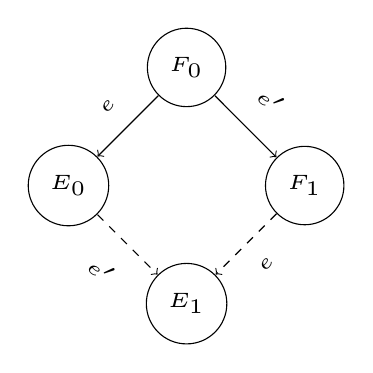
\begin{tikzpicture}[transform shape, scale=1.5]
    \tikzstyle{every node} = [shape=circle]
    \node (a) [draw] at (1, 2) {\tiny $F_0$};
    \node (b) [draw] at (0, 1) {\tiny $E_0$};
    \node (c) [draw] at (2, 1) {\tiny $F_1$};
    \node (d) [draw] at (1, 0) {\tiny $E_1$};
      \draw [->] (a) -- (c) node[pos=.5,sloped,above] {\tiny $e'$};
      \draw [->] (a) -- (b) node[pos=.5,sloped,above] {\tiny $e$};
      \draw [dashed, ->] (b) -- (d) node[pos=.5,sloped,below] {\tiny $e'$};
      \draw [dashed, ->] (c) -- (d) node[pos=.5,sloped,below] {\tiny $e$};
  \end{tikzpicture}
  \end{figure}
Contradiction: $E_1$ is both $0$- and $1$-valent.
\end{frame}

\begin{frame}{$p = p'$}
  Consider any finite deciding run from $F_0$ in which $p$ takes no steps, let $\sigma$ be the corresponding schedule and $A = \sigma(F_0)$.
\end{frame}

\begin{frame}{$p = p'$}
  \begin{figure}[!h]
  \centering
  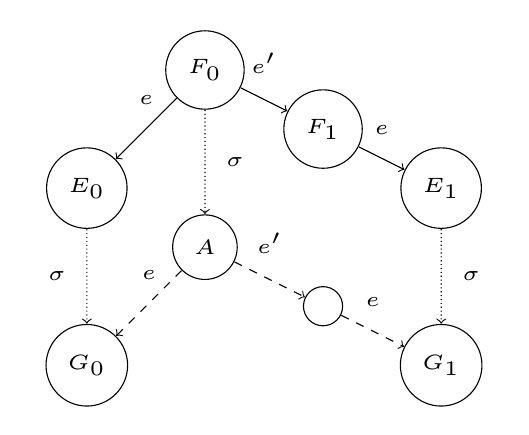
\begin{tikzpicture}[transform shape, scale=1.5]
    \tikzstyle{every node} = [shape=circle]
    \node (f0) [draw] at (1, 2.5) {\tiny $F_0$};
    \node (f1) [draw] at (2, 2) {\tiny $F_1$};
    \node (e1) [draw] at (3, 1.5) {\tiny $E_1$};
    \node (e0) [draw] at (0, 1.5) {\tiny $E_0$};
    \node (a)  [draw] at (1, 1) {\tiny $A$};
    \node (nn) [draw] at (2, .5) {};
    \node (g0) [draw] at (0, 0) {\tiny $G_0$};
    \node (g1) [draw] at (3, 0) {\tiny $G_1$};
    \draw [->] (f0) -- (e0) node[pos=.5, above] {\tiny $e$};
    \draw [->] (f0) -- (f1) node[pos=.5, above] {\tiny $e'$};
    \draw [->] (f1) -- (e1) node[pos=.5, above] {\tiny $e$};
    \draw [densely dotted, ->] (f0) -- (a) node[pos=.5, right] {\tiny $\sigma$};
    \draw [densely dotted, ->] (e0) -- (g0) node[pos=.5, left] {\tiny $\sigma$};
    \draw [densely dotted, ->] (e1) -- (g1) node[pos=.5, right] {\tiny $\sigma$};
    \draw [dashed, ->] (a) -- (g0) node[pos=.5, above] {\tiny $e$};
    \draw [dashed, ->] (a) -- (nn) node[pos=.5, above] {\tiny $e'$};
    \draw [dashed, ->] (nn) -- (g1) node[pos=.5, above] {\tiny $e$};
  \end{tikzpicture}
  \end{figure}
  Contradiction: the run to $A$ is deciding, but $A$ is bivalent! This concludes the case analysis and proves the lemma.
\end{frame}

\begin{frame}{Constructing an infinite non-deciding run}
  \begin{itemize}
    \item The message buffer is ordered by the time messages were sent.
    \item Organize the processes into a queue (initially in arbitrary order).
    \item The run will consist of an infinite sequence of stages each starting and ending in a bivalent configuration.
    \item At the beginning of each stage, consider the earliest pending message $m$ to $p_{head}$ (process at the head of the queue) or let $m = \varnothing$.
    \item Apply the delay lemma to $e=(p_{head}, m)$ and arrive to a bivalent configuration with $e$ applied last.
    \item Move $p_{head}$ to the tail of the queue.
  \end{itemize}
\end{frame}

\begin{frame}{Constructing an infinite non-deciding run}
  The sequence of stages constructed in this way from a bivalent initial configuration constitutes an admissible run which never decides on a value. In fact, this run has \alert{no faulty processes}.

  We have just proven
  \begin{theorem}[FLP impossibility]
    No consensus protocol is totally correct in spite of one fault.
  \end{theorem}
\end{frame}
%\begin{frame}{Interprocess communication}
%
%\end{frame}
%\begin{frame}{Atoi


\end{document}


